\documentclass[11pt, titlepage, twoside]{article}

\usepackage{graphicx}
\usepackage[margin=1in]{geometry}
\usepackage[hidelinks=true]{hyperref}
\usepackage[utf8]{inputenc}
\usepackage[english]{babel}
\usepackage[comma,authoryear,round]{natbib}
\usepackage{nopageno}
\usepackage{tocloft}
\usepackage{array}
\usepackage{booktabs}
\usepackage{authblk}
\usepackage{microtype}
\usepackage{charter}
\usepackage[nolist,nohyperlinks]{acronym}
\usepackage{siunitx}

\bibliographystyle{abbrvnat}

\graphicspath{{../figures/}}

\cftpagenumbersoff{figure}
\cftpagenumbersoff{table}

\renewcommand\Affilfont{\itshape\small}

\newcommand{\beginsupplement}{%
        \setcounter{table}{0}
        \renewcommand{\thetable}{S\arabic{table}}%
        \setcounter{figure}{0}
        \renewcommand{\thefigure}{S\arabic{figure}}%
     }

\acrodef{HURDAT2}{revised Atlantic hurricane database}
\acrodef{US}{United States}
\acrodef{NOAA}{National Oceanic and Atmospheric Administration}
\acrodef{CDC}{Centers for Disease Control}
\acrodef{UTC}{Coordinated Universal Time}
\acrodef{NHC}{National Hurricane Center}
\acrodef{NLDAS-2}{North American Land Data Assimilation System Phase 2}
\acrodef{WONDER}{Wide-ranging Online Data for Epidemiological Research}
\acrodef{FIPS}{Federal Information Processing Standard}
     
\frenchspacing



\begin{document}


\title{Supplemental Material for ``Assessing United States county-level
exposure for research on tropical cyclones and human health"}

\author[1,*]{G. Brooke Anderson} 
\author[1,2]{Joshua Ferreri}
\author[3]{Mohammad Al-Hamdan} 
\author[3]{William Crosson} 
\author[4]{Andrea Schumacher} 
\author[5]{Seth Guikema} 
\author[6]{Steven Quiring} 
\author[7]{Dirk Eddelbuettel} 
\author[1]{Meilin Yan} 
\author[8]{Roger D. Peng}

\affil[1]{Department of Environmental \& Radiological Health Sciences, Colorado 
  State University, Fort Collins, CO, 80523} 
\affil[2]{University of Colorado Anschutz Medical Campus, School of Medicine, Aurora, CO, 80045} 
\affil[3]{Universities Space Research Association, NASA Marshall Space Flight 
  Center, Huntsville, AL, 35805}
\affil[4]{Cooperative Institute for Research in the Atmosphere, Colorado State
  University, Fort Collins, CO, 80523} 
\affil[5]{Department of Industrial and Operations Engineering, University of 
  Michigan, Ann Arbor, MI, 48109}
\affil[6]{Department of Geography, Ohio State University, Columbus, OH, 43210}
\affil[7]{Department of Statistics, University of
  Illinois at Urbana-Champaign, Champaign, IL, 61820} 
\affil[8]{Department of Biostatistics, Johns Hopkins Bloomberg School of Public 
  Health, Baltimore, MD, 21205}
\affil[*]{Corresponding author: Brooke Anderson, brooke.anderson@colostate.edu}
        
\date{}

\maketitle

\beginsupplement

\begin{comment}

\begin{figure}[tbhp!]
\centering
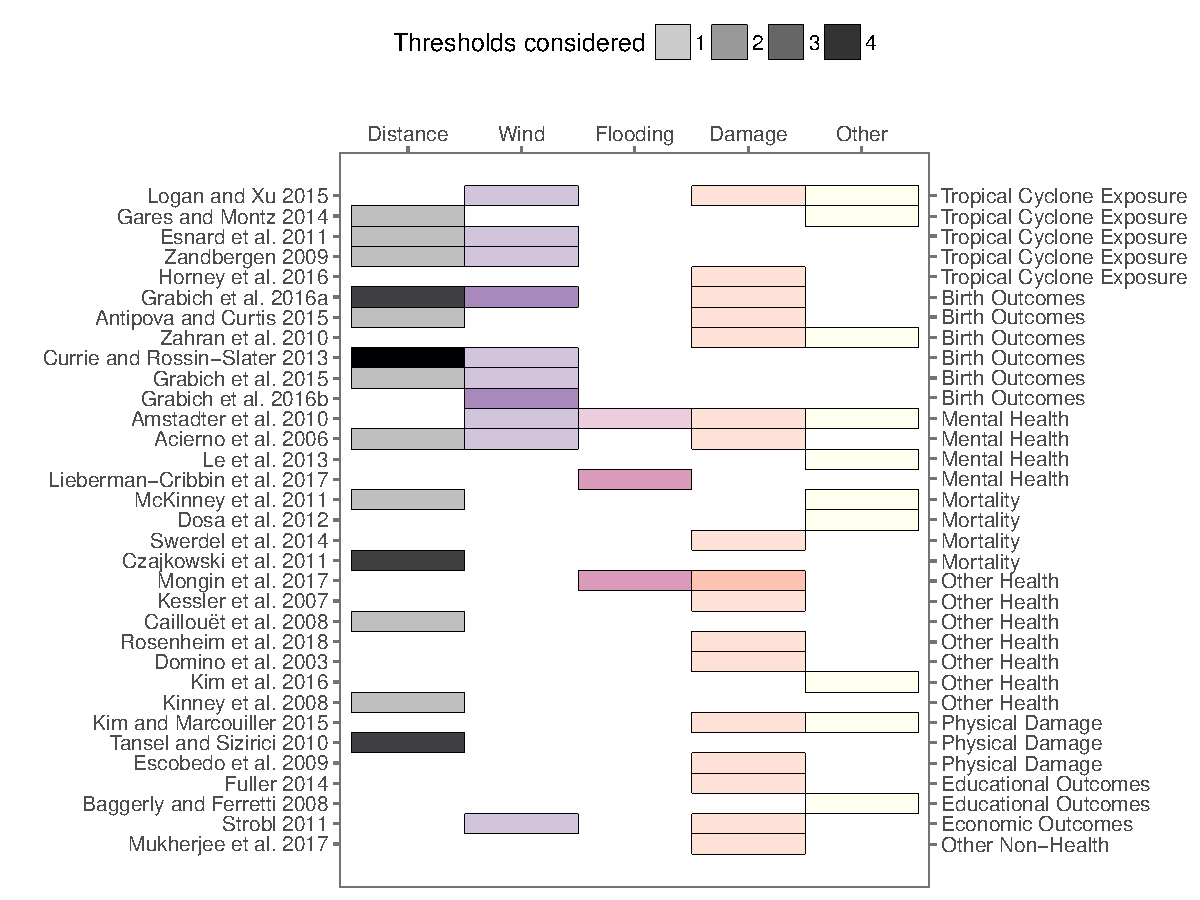
\includegraphics[width=\linewidth]{previous_exposure_metrics}
\caption{Metrics used in a sample of previous studies to assign exposure to
tropical cyclones in \ac{US}-based tropical cyclone exposure or impact studies.
Citations for each study are shown on the left and the broad topic of the study
on the left. Presence of a bar for a study-metric combination indicates that
the given metric was used in the study in assessing exposure to tropical
cyclones for that study, either alone or in combination with other metrics for
which that study has bars. The color transparency of each bar indicates the
number of different thresholds considered for defining storm exposure in the
study under that hazard (e.g., less transparent bars indicate that a study
considered multiple thresholds of the metric in defining tropical cyclone
exposure as a method of sensitivity analysis). Studies for which there are two
or more bars (e.g., bars for both distance and wind) indicate studies that
either used separate exposure assessments, one for each metric, (e.g., as a
sensitivity analysis) or used a single exposure index that incorporated
multiple metrics in its definition. ``Damage" often indicate use of Federal
Emergency Management Agency (FEMA) reports, although occasionally used damage
reports from other sources, including newspaper reports. Examples of ``Other"
include evacuation orders, excessive school closures, length of time a storm
was near a location, and detailed, holistic analyses of a specific storm or
storms. References for each study are included in the bibliography of this
Supplemental Material.}
\label{fig:previousmetrics}
\end{figure}

\nocite{logan2015, gares2014, esnard2011, zandbergen2009, horney2016,
grabich2016, antipova2015post, zahran2010, currie2013, grabich2015,
grabich2016hurricane, amstadter2010, acierno2006, le2013, lieberman2017,
mckinney2011, dosa2012evacuate, swerdel2014, czajkowski2011, mongin2017,
kessler2007hurricane, caillouet2008increase, rosenheim2018disaster,
domino2003disasters, kim2016, kinney2008, kim2015, tansel2010, escobedo2009,
fuller2014, baggerly2008impact, strobl2011economic, mukherjee2017}

\newpage

\end{comment}

\begin{figure}[tbhp!]
\centering
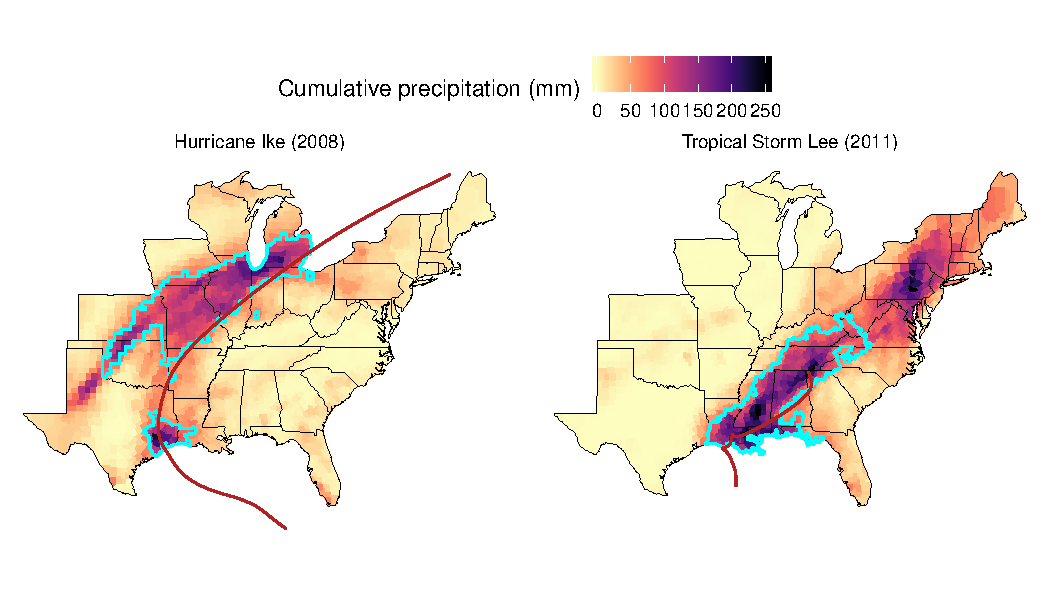
\includegraphics[width=0.9\linewidth]{rainexamples}
\caption{Examples of storms where some storm-related rainfall occured
         500 \si{\kilo\metre} or further from the storm's track. 
	 The red line on each map shows the track of the storm. 
	 The color of each county in the map gives the cumulative 
	 precipitation in the county from two days before to one day after
	 the storm's closest approach (in \si{\milli\metre}). The blue 
	 outline identifies the collection of counties
	 that were classified as ``exposed" based on the rainfall exposure 
	 criteria (Table 1 of main text), which includes the constraint
	 that the storm must have come within 500 \si{\kilo\metre} of the 
	 county. }
\label{fig:rainexamples}
\end{figure}

\clearpage 

\begin{figure}[tbhp!]
\centering
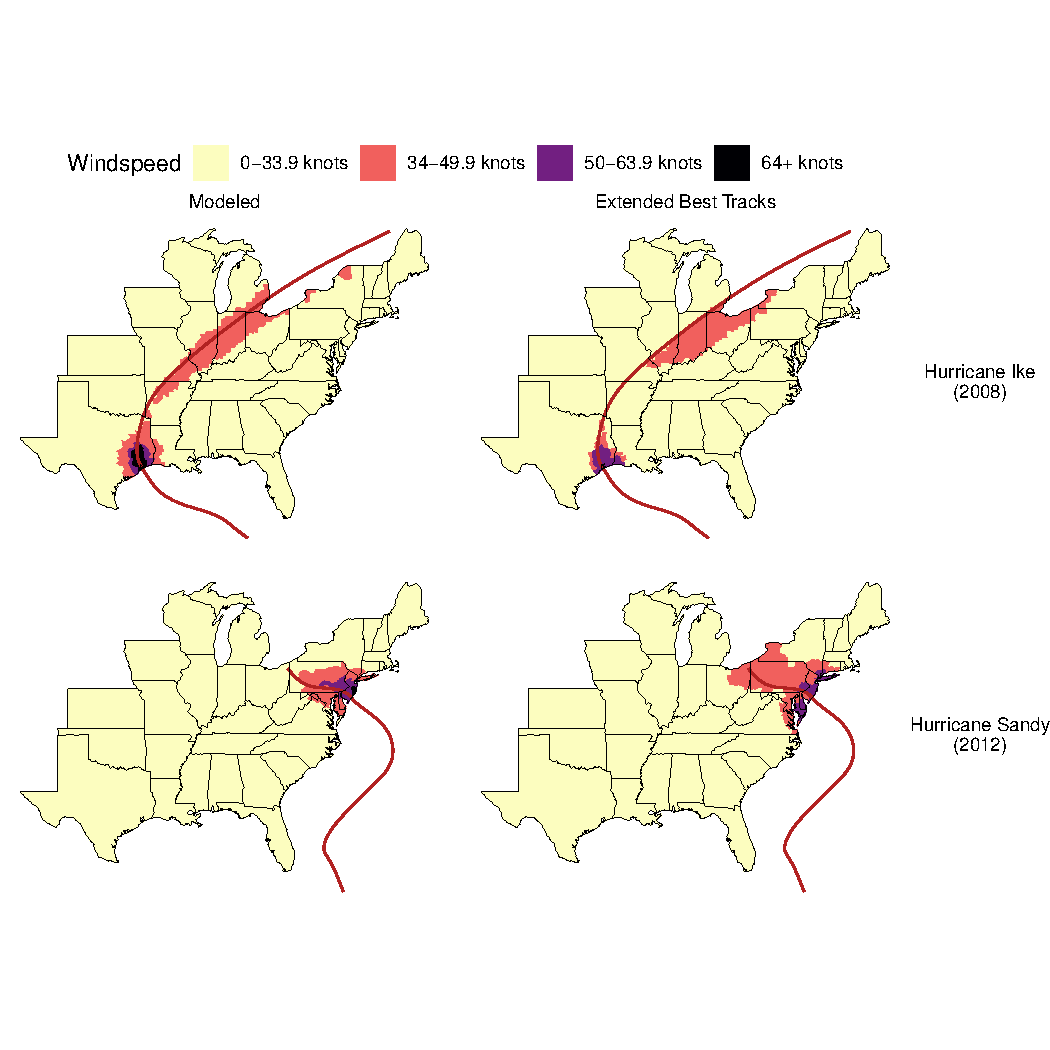
\includegraphics[width=\linewidth]{windexamples}
\caption{Comparison of county-level estimates of peak sustained surface wind 
	for Hurricane Ike in 2008 (top) and Hurriance Sandy in 2012 (bottom). 
	Each map shows the estimated peak sustained surface wind 
	classification ($<$34~kt; 34\,--\,49.9~kt; 
	50\,--\,63.9~kt; $\ge$64~kt) for each study county. 
	The maps labelled ``Modeled'' (left)
	shows the classifications based on modeled peak sustained surface wind,
	which were included in the open-source data as the main 
	wind metric and used in further analysis in this research. The maps
	labelled ``Extended Best Tracks'' (right) show classifications based on the 
	wind radii given in \ac{HURDAT2} (included as a secondary wind 
	metric in the open-source data). The red lines show the storms' 
	tracks.
	}
\label{fig:windexamples}
\end{figure}

\clearpage

\begin{figure}[tbhp!]
\centering
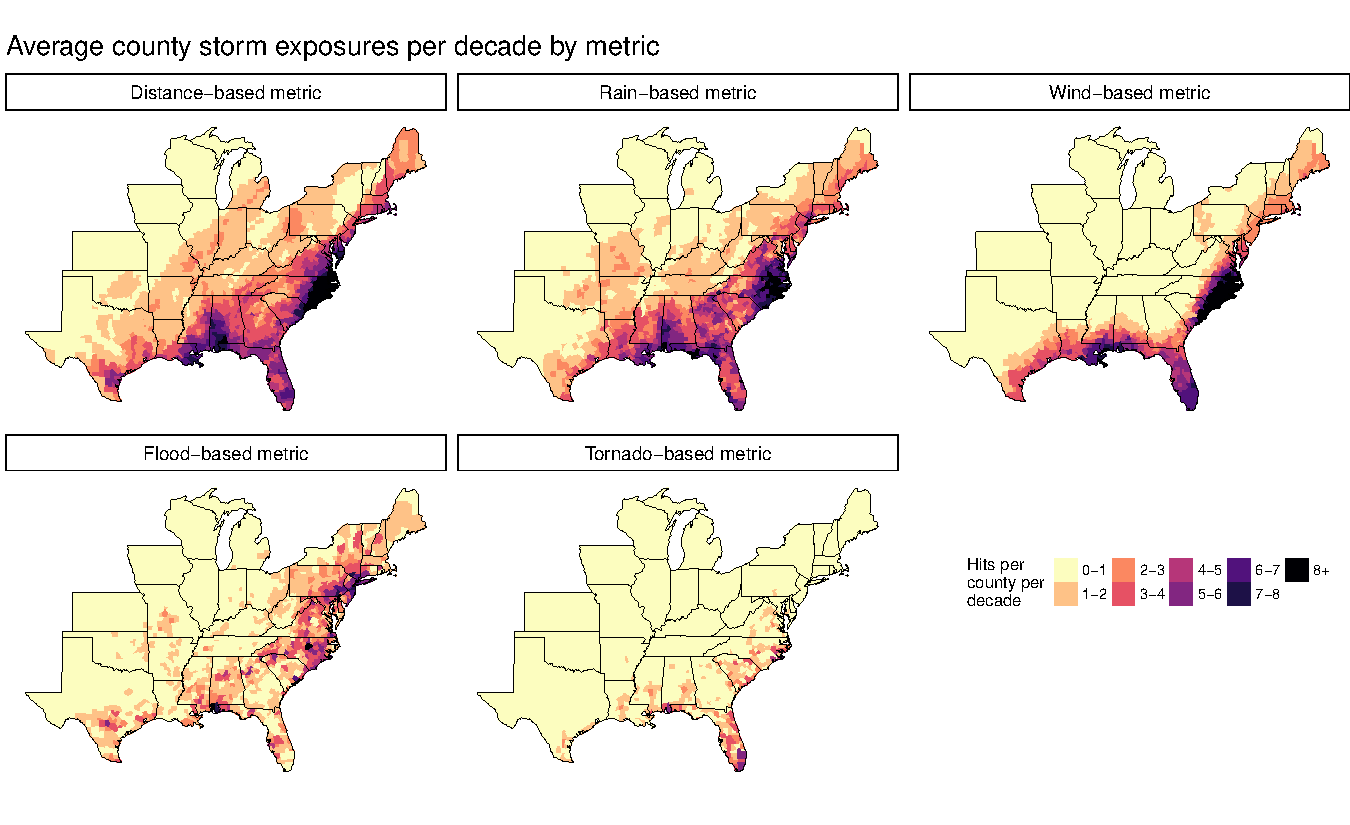
\includegraphics[width=7cm]{averageexposureonlysupp}
\caption{Average number of storm exposures per decade in U.S. counties for each 
	single-hazard exposure metric, limited analysis to years for which data on all five 
	exposures were available (1996\,--\,2011). The criteria behind each of 
	the five metrics is given in Table 1 of the main text. 	
	} 
\label{fig:averageexposuresupp}
\end{figure}

\clearpage 

\begin{figure}[tbhp!]
\centering
\includegraphics[width=\linewidth]{othertopstorms}
\caption{Differences in the counties assessed as ``exposed'', based on different
	exposure metrics, for a sample of storms. These sample storms were 
	selected as the  storms with largest extent (as measured by the 
	number of counties exposed based on any metric) from each of the 
	clusters shown in the Jaccard heatmap in the main text (Figure 7).}
\label{fig:othertopstorms}
\end{figure}

\clearpage

\begin{comment}

\begin{figure}[tbhp!]
\centering
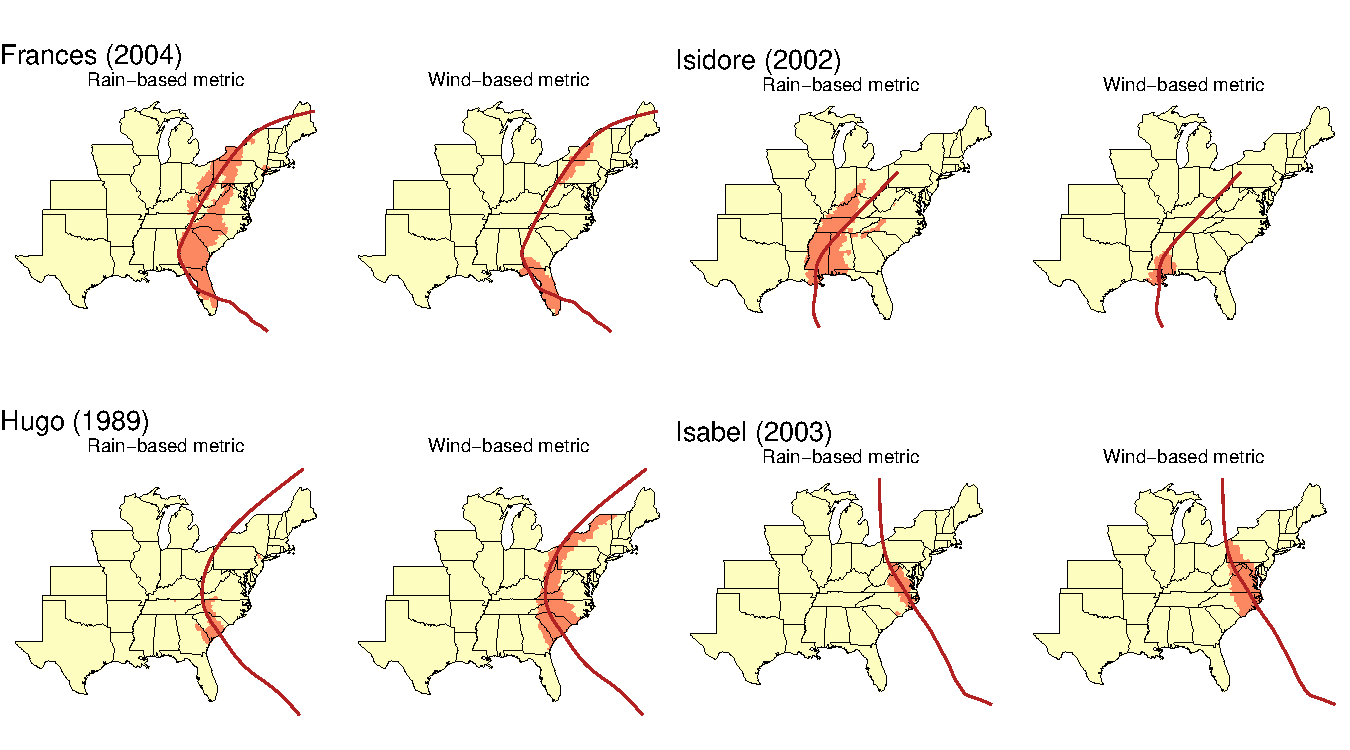
\includegraphics[width=\linewidth]{extentdisagreement}
\caption{Examples of storms for which exposure assessments differed
	substantially between rain-based and wind-based metrics. Counties 
	shown in orange were classified as exposed to a given storm by a 
	given metric; those in yellow were classified as not exposed. 
	The storm's track is shown in red. For both Frances (2004) and 
	Isidore (2002) (top panel), substantially more counties were assessed 
	as exposed when measuring exposure based on rain rather than wind. 
	Conversely, for both Hugo (1989) and Isabel (2003) (bottom panel), 
	substantially more counties were assessed as exposed based on wind 
	compared to rain.}
\label{fig:extentdisagreement}
\end{figure}

\clearpage

\end{comment}

\printbibliography

\end{document}

